% Documentatie Herfstkamp project: Bouw van een audio-versterker
% Jules Hammenecker
% Vrije Universiteit Brussel - Dept. ELEC
% Augustus 2015

\newif\ifoplossing

% Comment to choose between versions
%\oplossingfalse
\oplossingtrue


\ifoplossing
\title{Project Ingenieurswetenschappen: \\ Elektronisch ontwerp van de e-VUBOX~speaker\\ Oplossingen}

\else
\title{Project Ingenieurswetenschappen: \\ Elektronisch ontwerp van de e-VUBOX~speaker\\ Invulblad}

\fi


\author{Vrije Universiteit Brussel}
\date{Versie 08.2015}

\documentclass{article}
	\usepackage[a4paper]{geometry}
	%\usepackage[utf8x]{inpudetenc}
	\usepackage[T1]{fontenc}
	\usepackage[dutch]{babel}
	\usepackage{amsmath}
\usepackage{pdflscape}
	\newtheorem{DIY}{Doe-het-zelf}
\usepackage{multicol}
	%%% FIGURES %%%
	\usepackage[pdftex]{graphicx}
	\usepackage{caption,subcaption}
	\usepackage{hyperref}
	\graphicspath{ {./figs/} }




\begin{document}
	
	\maketitle

	\tableofcontents
	\clearpage

	\section{Basis Elektronica}
	\subsection{De weerstand}
			\begin{figure}[h!]
				\centering
				\includegraphics{vbweerstand.pdf}
				\caption{Voorbeeldnetwerkje.}
				\label{fig:vbweerstand}
			\end{figure}

			\begin{DIY} 
			\begin{align*}
				\text{Wet van Ohm:}~&V = R\cdot I \\
				\text{Vermogen:}~&P = V\cdot I \\
			\end{align*}
			\ifoplossing
				\begin{align*}
				    I &= V/R \\ &= 230~V/80~\Omega = 2.875 A \\
				    P &= V \cdot I = V^2/R \\ &= (230~V)^2/80~\Omega = 661.25~W \\
				    I&= 2.875~A \hspace{10em}P=  661.25~W 
				\end{align*}
			\else
				~\vspace{20ex}
				\begin{align*}
			    I&= \ldots & P&= \ldots 
				\end{align*}
			\fi



			
			\end{DIY}

	\subsection{Netwerken}

			\begin{figure}[h!]
				\centering
				\begin{subfigure}[b]{0.45\linewidth}
					\centering
					\includegraphics{kcl_oef.pdf}
					\caption{Vind $I_R$ en $I_s$.}
					\label{subfig:kcl_oef}
				\end{subfigure}
				~
				\begin{subfigure}[b]{0.45\linewidth}
					\centering
					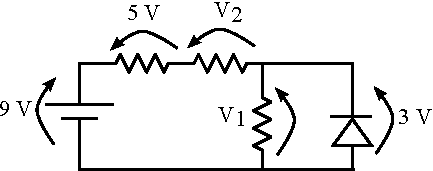
\includegraphics[width=\linewidth]{kvl_oef.pdf}
					\caption{Vind $V_R$ en $U_C$. }
					\label{subfig:kvl_oef}
				\end{subfigure}
			\caption{De wetten van Kirchhoff}
			\label{fig:kirchoff_oef}
			\end{figure}

			\begin{DIY}
			\ifoplossing

			\begin{align*}
			\intertext{Stroomwetten:}
			    &I_S = 0.05A + I_R \\
			    &I_R + 0.05A -0.2A = 0 \\
			 \intertext{Oplossing:}
			 &I_R = 0.2A - 0.05A = 0.15A \\
			 &I_S = 0.05A + 0.15A = 0.2 A
			\end{align*}

			\begin{align*}
			\intertext{Spannigswetten:}
			    &V_1-3V = 0 \\
			    &9V-5V-V_2-V_1 = 0 \\
			 \intertext{Oplossing:}
			 &V_1 = 3V \\
			 &V_2 = 9V-5V-3V = 1V
			\end{align*}

			\begin{align*}
			    I_S &= 0.15~A & V_1 = 3~V\\
			    I_R &= 0.05~A  & V_2 =1~V 
			\end{align*}
			\else
			~\vspace*{20ex}


			\begin{align*}
			    I_S &= \ldots & V_1 = \ldots\\
			    I_R &= \ldots & V_2 =\ldots
			\end{align*}
			\fi



			
			
			\end{DIY}


\section{Bouwstenen}
\subsection{Volumeknop}

			\begin{figure}[h!]
				\centering
				\includegraphics{weerstandsdeler}
				\caption{Volumeregeling: de spanningsdeler}
				\label{fig:volume}
			\end{figure}

			\begin{DIY}

				\ifoplossing
				\begin{align*}
					\intertext{Shortcut met serieweerstand:}
					   V_1 &= R_1 \cdot I_1 = R_1 \cdot \frac{V_S}{R_1+R_2}
					\intertext{Lange weg:}
					 V_1 &= R_1 \cdot I_1 \\
					 V_1 &= R_1 \cdot I_2 \\
					 V_1 &= R_1 \cdot \frac{V_2}{R_2} \\
					 V_1 &= R_1 \cdot \frac{V_S-V_1}{R_2} \\
					 (1+\frac{1}{R_2}) V_1 &= R_1 \cdot \frac{V_S}{R_2} \\
					 V_1 &= \frac{R_1}{R_2} \cdot (\frac{R_2}{R_1+R_2}) V_S \\
					 V_1 &= \frac{R_1}{R_1+R_2} \cdot V_S
				\end{align*}
				\else	
					~\vspace*{20ex}
				\begin{align*}
				    V_1 = \ldots\ldots
				\end{align*}
				\fi			

			\end{DIY}

			\begin{DIY}

				\ifoplossing
					\begin{align}
					    \frac{R_1}{R_1+R_2} &= \frac{1.5V}{9V} \\
					    \frac{1 k\Omega}{1k\Omega + R_2} &= \frac{1}{6}\\
					    \frac{1k\Omega + R_2}{1 k\Omega} &= 6\\
					    R_2 &= 6 \cdot 1 k\Omega - 1 k\Omega =  5 k\Omega  \\
					    \intertext{maar deze waarde is geen E12-waarde, we kiezen dus:}
					    R_2 &= 4.7 k\Omega
					\end{align}
				\else
					~\vspace*{20ex}
					\begin{align*}
					    R_2 = \ldots\ldots
					\end{align*}
				\fi
					
			\end{DIY}

			\begin{DIY}

			\ifoplossing
				\begin{align*}
					P &= V \cdot I = V^2 / R_{pot} \\
					R_{pot} &= (200mW)/4\mu W \\
				    R_{pot} &= 10 k\Omega
				\end{align*}
			\else
				~\vspace*{20ex}
				\begin{align*}
				    R_{pot} = \ldots\ldots
				\end{align*}
			\fi

			\end{DIY}	

\subsection{Statusledje}
			\begin{figure}[htbp]
				\centering
				\includegraphics{diode_netwerk}
				\caption{Diode netwerk.}
				\label{fig:diode_netwerk}
			\end{figure}

			\begin{DIY} 

			\ifoplossing
				\begin{align*}
				\intertext{Kirchhoff:}
					V_S &- U_D - V_R = 0 \\
					I_S &= I_D = I_R \\
				\intertext{De weerstand die nodig is:}	
				    R_{led} &= \frac{V_R}{I_R} \\
				    		&= \frac{V_S-U_D}{I_D} \\
				    		&= \frac{9V-1.8V}{10mA} \\
				    		&= \frac{7.2V}{10mA} = 720 \Omega \\
				\intertext{We kiezen een weerstand in de E12 reeks:}
				    R_{led} &= 680 \Omega
				\end{align*}
			\else
				~\vspace*{20ex}
				\begin{align*}
				    R_{led} = \ldots\ldots
				\end{align*}
			\fi

			\end{DIY}

\subsection{Versterker}
		\begin{figure}[h!]
					\centering
					\includegraphics{ges}
					\caption{Versterkerschakeling met de transistor.}
					\label{fig:ges}
				\end{figure}
			\begin{DIY}	
				\ifoplossing
					\begin{align*}
					    I_C + I_B + I_E &= 0 \\
					    I_C + \frac{I_C}{\beta} + I_E &= 0 \\
					    (1+\frac{1}{\beta})I_C +I_E &= 0\\
						\intertext{stel dat $\beta$ 1000 is en rond af:}   
						I_C \approx -I_E \\
					\end{align*}
				\else
					~\vspace*{20ex}
					\begin{align*}
						I_C \approx \ldots \ldots
					\end{align*}
				\fi


			\end{DIY}


			\begin{DIY} 
				\ifoplossing
					\begin{align*}
					    V_C &= V_{CC} - V_{R_C} \\
					    V_C &= V_{CC} - R_C \cdot I_C \\
					    V_C &= V_{CC} + R_C \cdot I_E \\
					    V_C &= V_{CC} - R_C \cdot \frac{V_E}{R_E} \\
					    V_C &= V_{CC} - \frac{R_C}{R_E} \cdot V_E \\
					    V_C &= V_{CC} - \frac{R_C}{R_E} \cdot(V_B - 0.7 V) 
					\end{align*}
				\else
					~\vspace*{60ex}
					\begin{align}
					    V_C = \ldots \ldots \ldots \ldots  \ldots  \ldots 
					\end{align}
				\fi

			\end{DIY}

			\begin{DIY} 	
			~\vspace*{20ex}
				\begin{align}
				    R_C &= \ldots \\
				    R_E &= \ldots
				\end{align}
			\end{DIY}	

			\begin{DIY} 
			~\vspace*{20ex}
				\begin{align}
					V_B &= \ldots \\
				    R_1 &= 1k\Omega \\
				    R_2 &= \ldots
				\end{align}
			\end{DIY}	


\begin{landscape}
	
\section{Overzicht}
		\begin{figure}[htbp]
		%	\centering
			\includegraphics[width=\linewidth]{volledig_schema}
			\caption{Volledig Schema}
			\label{fig:volledig_schema}
		\end{figure}
\end{landscape}
\end{document}